\begin{figure*}[t]\centering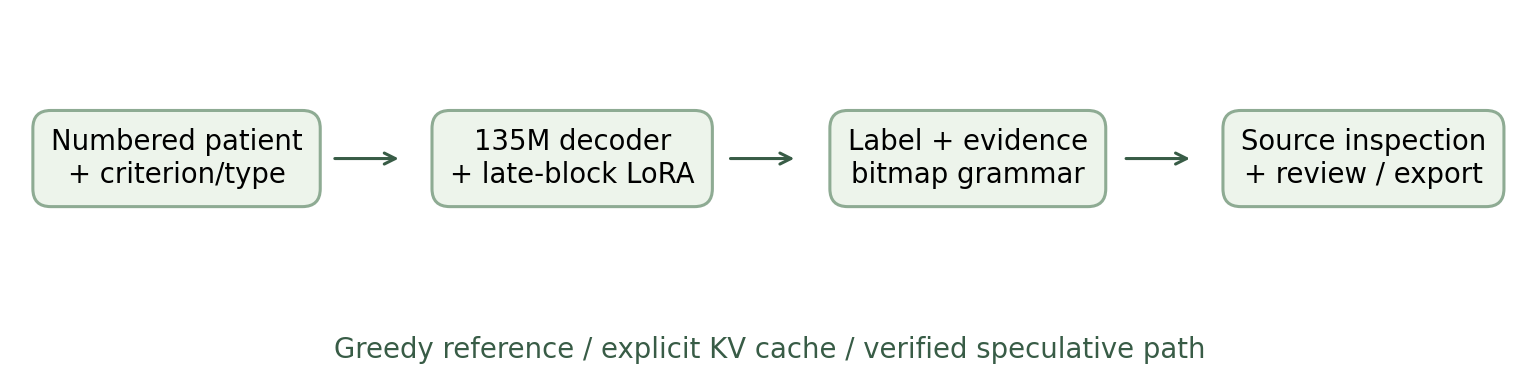
\includegraphics[width=\textwidth]{workflow.png}\caption{Screening workflow. All decoding modes share the target model; the evidence parser preserves source sentence IDs.}\label{fig:workflow}\end{figure*}

Figure~\ref{fig:workflow} summarizes the application path. The full experiments use 603 training annotations; development smoke runs are archived separately and are not reported as final results.

The original CPU automated suite reports 16 passing checks. These cover attention agreement, cached/uncached/speculative token equality, cache growth, full-acceptance and rejection branches, early stopping, structured masks, evidence empty-set conventions, data isolation, response-loss equivalence, frozen base weights, truncation and application input/export handling.

\begin{table}[t]\centering\small\caption{Selected training configuration and observed preprocessing.}\label{tab:training}\begin{tabular}{lr}\toprule Setting & Value\\\midrule

Target parameters & 134,607,168\\

Trainable parameters & 92,160\\

Selected epoch & 3\\

Best validation loss & 0.3446\\

Three-epoch elapsed time & 55.13 min\\

Train truncated records & 0\\

Validation truncated records & 0\\

Test truncated records & 0\\\bottomrule\end{tabular}\end{table}

\begin{figure}[t]\centering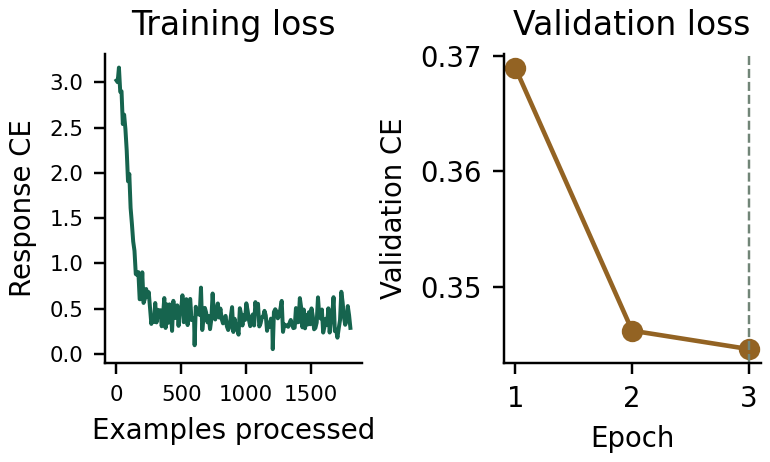
\includegraphics[width=\columnwidth]{training.png}\caption{Measured training and validation response loss. The dashed line marks the selected epoch.}\label{fig:training}\end{figure}

Table~\ref{tab:training} records the selected adapter. Validation loss changed from 0.3690 after epoch one to 0.3446 after epoch three (Fig.~\ref{fig:training}). Selection uses the minimum validation loss, not the final test score. Training loss windows are descriptive and are not an unbiased epoch-average curve.

\begin{table}[t]\centering\small\caption{Validation comparison. Acc=accuracy; MF=macro-F1; EF=evidence micro-F1.}\label{tab:validation}\begin{tabular}{llrrr}\toprule Model & Criteria & Acc & MF & EF\\\midrule

base & overall & 0.199 & 0.148 & 0.157\\

base & inclusion & 0.530 & 0.177 & 0.417\\

base & exclusion & 0.043 & 0.047 & 0.093\\

adapted & overall & 0.641 & 0.273 & 0.155\\

adapted & inclusion & 0.470 & 0.234 & 0.234\\

adapted & exclusion & 0.721 & 0.210 & 0.000\\

\bottomrule\end{tabular}\end{table}

\begin{table}[t]\centering\small\caption{Held-out comparison. Acc=accuracy; MF=macro-F1; EF=evidence micro-F1.}\label{tab:test}\begin{tabular}{llrrr}\toprule Model & Criteria & Acc & MF & EF\\\midrule

base & overall & 0.233 & 0.155 & 0.176\\

base & inclusion & 0.347 & 0.135 & 0.305\\

base & exclusion & 0.168 & 0.099 & 0.096\\

adapted & overall & 0.612 & 0.259 & 0.145\\

adapted & inclusion & 0.467 & 0.220 & 0.196\\

adapted & exclusion & 0.695 & 0.205 & 0.000\\

\bottomrule\end{tabular}\end{table}

Tables~\ref{tab:validation} and~\ref{tab:test} compare identical examples and grammar settings before and after adaptation. Held-out accuracy changes from 0.233 to 0.612, while macro-F1 changes from 0.155 to 0.259. These measures must be interpreted together: frequent-label success can raise accuracy while rare classes remain poorly recognized. The results do not establish clinical reliability.

A diagnostic majority-label reference chooses the most frequent training label separately for each criterion type, with no test-derived choice. It obtains held-out accuracy 0.626 and macro-F1 0.226. This simple reference contextualizes the adapted model: improvement over an unadapted decoder does not by itself demonstrate strong clinical discrimination. The reference performs no evidence retrieval.

Evidence micro-F1 changes from 0.176 before adaptation to 0.145 afterwards. A label-accuracy gain therefore must not be described as a general evidence-quality gain. Many zero evidence flags and imbalanced label frequencies are plausible contributors, but this study does not establish their causal effect through an ablation.

The actual prediction distribution is inclusion: included (21), not enough information (54); exclusion: not excluded (131). No sentence was cited in 181 of 206 test records. Thus syntactic preservation of all six labels must not be confused with successful recognition of all six classes. The concentration on frequent outcomes and weak evidence selection are substantive failures of the adapted matcher. Verified inference mechanisms do not establish clinical reasoning quality.

\begin{table}[t]\centering\scriptsize\caption{Adapted model: held-out per-class classification. All six labels remain distinct.}\label{tab:classes}\begin{tabular}{lrrrr}\toprule Label & Prec. & Recall & F1 & N\\\midrule

included & 0.286 & 0.222 & 0.250 & 27\\

not included & 0.000 & 0.000 & 0.000 & 7\\

excluded & 0.000 & 0.000 & 0.000 & 0\\

not excluded & 0.695 & 1.000 & 0.820 & 91\\

not enough information & 0.537 & 0.439 & 0.483 & 66\\

not applicable & 0.000 & 0.000 & 0.000 & 15\\

\bottomrule\end{tabular}\end{table}

\begin{figure*}[t]\centering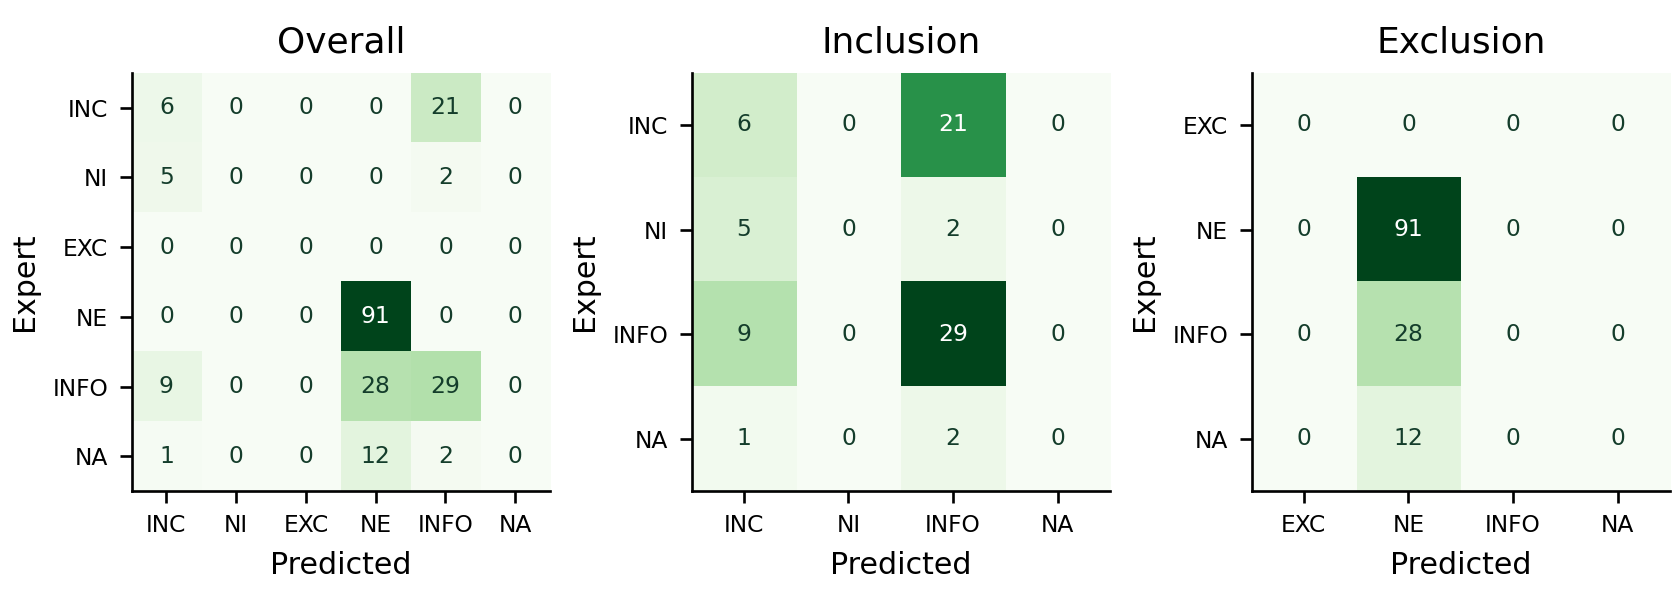
\includegraphics[width=\textwidth]{confusion.png}\caption{Adapted held-out confusion matrices. Rows are expert labels and columns are predictions. INC=included; NI=not included; EXC=excluded; NE=not excluded; INFO=not enough information; NA=not applicable.}\label{fig:confusion}\end{figure*}

Table~\ref{tab:classes} and Fig.~\ref{fig:confusion} expose minority-class errors that overall accuracy obscures. Zero-support classes remain in the specified macro denominator. Per-type per-class results and both base/adapted confusion matrices are also saved in the machine-readable metric files.

\begin{table}[t]\centering\scriptsize\caption{Adapted held-out evidence retrieval. Both-empty pairs score one per record, but contribute no pooled counts.}\label{tab:evidence}\begin{tabular}{lrrrrrr}\toprule & \multicolumn{3}{c}{Micro} & \multicolumn{3}{c}{Macro}\\Group & P & R & F1 & P & R & F1\\\midrule

overall & 0.300 & 0.096 & 0.145 & 0.690 & 0.694 & 0.691\\

inclusion & 0.300 & 0.145 & 0.196 & 0.362 & 0.373 & 0.364\\

exclusion & 0.000 & 0.000 & 0.000 & 0.878 & 0.878 & 0.878\\

\bottomrule\end{tabular}\end{table}

Table~\ref{tab:evidence} includes 134 test records where both evidence sets are empty. Differences between micro and macro scores reflect both citation-set sizes and the explicit empty-set convention. Evidence scores assess localization; they do not prove that cited sentences logically entail the model label.

\begin{table*}[t]\centering\small\caption{Adapted CPU decoding measurements. Median of three repetitions after one warmup; peak RSS is a fresh-process high-water mark including loaded model(s).}\label{tab:decode}\begin{tabular}{rrlrrrrr}\toprule Input & Output & Path & Prefill (s) & Decode (s) & Total (s) & Tokens/s & Peak RSS (MiB)\\\midrule

32 & 8 & uncached & 0.212 & 1.278 & 1.481 & 5.40 & 1206.2\\

32 & 8 & cached & 0.140 & 0.576 & 0.732 & 10.92 & 1206.2\\

32 & 8 & speculative & 0.183 & 2.407 & 2.591 & 3.09 & 1748.4\\

128 & 16 & uncached & 0.375 & 6.694 & 7.051 & 2.27 & 1206.9\\

128 & 16 & cached & 0.401 & 1.523 & 1.945 & 8.23 & 1206.8\\

128 & 16 & speculative & 0.520 & 5.044 & 5.644 & 2.83 & 1748.1\\

256 & 32 & uncached & 0.884 & 31.163 & 32.212 & 0.99 & 1206.7\\

256 & 32 & cached & 0.859 & 3.012 & 3.891 & 8.22 & 1206.1\\

256 & 32 & speculative & 1.019 & 10.878 & 12.126 & 2.64 & 1748.5\\

\bottomrule\end{tabular}\end{table*}

\begin{figure}[t]\centering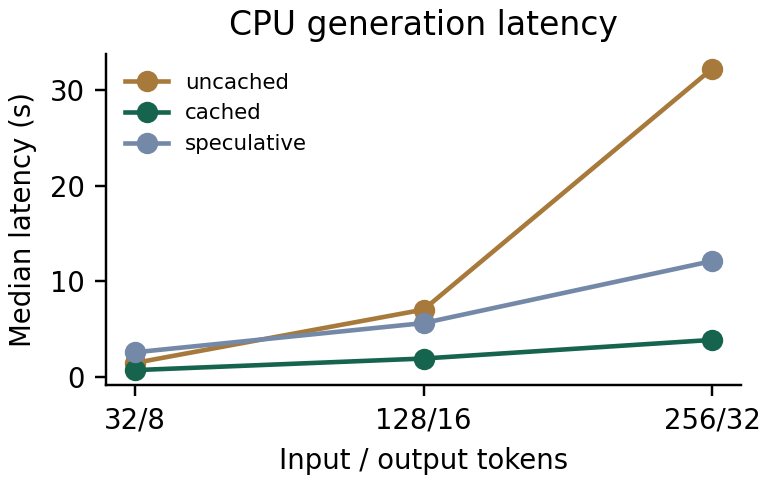
\includegraphics[width=\columnwidth]{latency.png}\caption{Measured end-to-end generation latency, including prefill.}\label{fig:latency}\end{figure}

Token-level agreement across all three final length pairs is verified. Table~\ref{tab:decode} and Fig.~\ref{fig:latency} separate prefill from incremental decoding. Caching avoids repeated prefix computation but retains KV memory. Process RSS includes fixed framework and weight costs, so it is not an isolated cache-size measure.

Across the measured length pairs, cached generation is 2.02--8.28 times as fast as the uncached reference by median end-to-end latency. These ratios apply to this target, CPU, prompt family and output budgets; they are not universal model speedups.

\begin{table}[t]\centering\scriptsize\caption{Speculative acceptance and speed relative to ordinary cached greedy. Speedup below one means slower.}\label{tab:spec}\begin{tabular}{rrrr}\toprule Input/output & Accepted/proposed & Acceptance & Speedup\\\midrule

32/8 & 0/26 & 0.000 & 0.283\\

128/16 & 2/54 & 0.037 & 0.345\\

256/32 & 2/114 & 0.018 & 0.321\\

\bottomrule\end{tabular}\end{table}

Table~\ref{tab:spec} reports proposal counts from the first deterministic run and the median latency ratio. Low acceptance requires repeated draft forwards and target corrections. A smaller model is therefore insufficient by itself to guarantee acceleration. The pruned draft is a practical memory experiment with limited calibration, and the measured ratios bound claims about its usefulness.

\begin{table}[t]\centering\scriptsize\caption{Educational attention measurements (batch 1, heads 3, width 32). Error is against the dense reference.}\label{tab:attention}\begin{tabular}{rlrrr}\toprule Length & Path & Time (ms) & Max error & RSS MiB\\\midrule

64 & reference & 0.302 & 0.0e+00 & 395.1\\

64 & tiled & 1.986 & 3.6e-07 & 395.5\\

128 & reference & 1.425 & 0.0e+00 & 396.3\\

128 & tiled & 9.197 & 3.0e-07 & 395.6\\

256 & reference & 2.307 & 0.0e+00 & 398.9\\

256 & tiled & 17.209 & 6.0e-07 & 396.2\\

512 & reference & 7.926 & 0.0e+00 & 412.7\\

512 & tiled & 84.642 & 4.8e-07 & 396.2\\

\bottomrule\end{tabular}\end{table}

Table~\ref{tab:attention} shows a maximum tiled numerical error of 5.96e-07; the largest mean error is 2.79e-08. The logical score tile stays at most 0.0117 MiB, whereas the dense score tensor reaches 3.00 MiB. These buffer estimates exclude other intermediates and are not claimed as peak process-memory savings. Python loops and small tensor dispatch can outweigh tiling benefits on CPU.

At sequence length 512, the tiled implementation takes 84.642 ms versus 7.926 ms for dense attention. This directly measures the educational implementation, not a fused FlashAttention kernel.

\begin{table*}[t]\centering\scriptsize\caption{Eight distinct adapted-model held-out error cases. Full notes, IDs, gold and predicted evidence are preserved in the error-analysis file.}\label{tab:errors}\begin{tabular}{rp{4.4cm}p{2.1cm}p{2.1cm}p{4.2cm}}\toprule ID & Criterion (abbreviated) & Expert label & Prediction & Observed error\\\midrule

160 & Patient willing to give full informed consent for participation & included & included & extra citation, missed citation\\

161 & Patients undergoing elective carotid endarterectomy & not included & included & missed inclusion conflict, extra citation\\

165 & Pregnancy & not applicable & not excluded & applicability confusion\\

169 & Patients with an estimated pre-operative glomerular filtration rate \(<\) 30mls/min/1.73m2 & not enough information & not excluded & unsupported certainty\\

179 & Had been performed central venous puncture or catheterization before. & not excluded & not excluded & missed citation, empty predicted evidence\\

185 & Patients were included if they were diagnosed with Shock, Acute respiratory distress syndrome (ARDS), or both. & included & not enough information & over-abstention, missed citation, empty predicted evidence\\

304 & Patients of both sexes aged \(\geq\) 18 years. & included & not enough information & over-abstention, missed citation, empty predicted evidence\\

381 & Age \(>\) 18 years at the time of signing the informed consent form & included & not enough information & over-abstention, missed citation, empty predicted evidence\\

\bottomrule\end{tabular}\end{table*}

Table~\ref{tab:errors} distinguishes label errors from sentence-localization errors. Unsupported certainty is defined relative to an expert insufficient-information label, not an independently established medical diagnosis. Extra/missed citations compare source-ID sets. The cases show why a valid citation ID and a grammatical output cannot establish factual support. The full error log retains contradictory expert/model outcomes and source text for individual review.

Annotation 161 is an unsupported positive result: the criterion specifies elective carotid endarterectomy, whereas cited sentence 0 describes cardiac catheterization. The citation is a valid source location but does not state the required procedure. This demonstrates the gap between source-ID validity and criterion entailment.

Annotation 169 asks about a pre-operative renal-filtration threshold. The supplied note contains no such measurement. The expert label is insufficient information, but the model returns not excluded with no citation. The app flags the absent evidence for review; the predicted negative outcome must not be read as proof that the threshold is not met.

Annotation 185 combines under-recognition and failed localization. The experts associate the inclusion criterion with sentences 2 and 3, which report observations and vital signs; the model instead abstains and retrieves neither sentence. The error concerns the benchmark expert judgment, not an independent clinical diagnosis made by this system.

\begin{table}[t]\centering\scriptsize\caption{Supplementary synthetic probes. These are not benchmark labels and are excluded from accuracy/F1.}\label{tab:stress}\begin{tabular}{p{2.5cm}p{3.1cm}l}\toprule Probe & Model output & Cited IDs\\\midrule

Conflicting ages & not enough information & []\\

Missing kidney data & not excluded & []\\

Explicit negation & included & [0]\\

\bottomrule\end{tabular}\end{table}

Table~\ref{tab:stress} tests three deliberately constructed situations after protocol freeze. The conflicting-age record contains both 52 and 72 years without resolving the discrepancy; citing a single age cannot resolve that contradiction. The missing-kidney-information case provides no renal measurement; a definite category would not establish that missing fact. The negation case distinguishes a condition mention from its presence. These probes illustrate behaviors for human review, not additional ground-truth benchmark performance or a basis for retuning.

\subsection{Final Browser Workflow Verification}

\begin{figure*}[t]\centering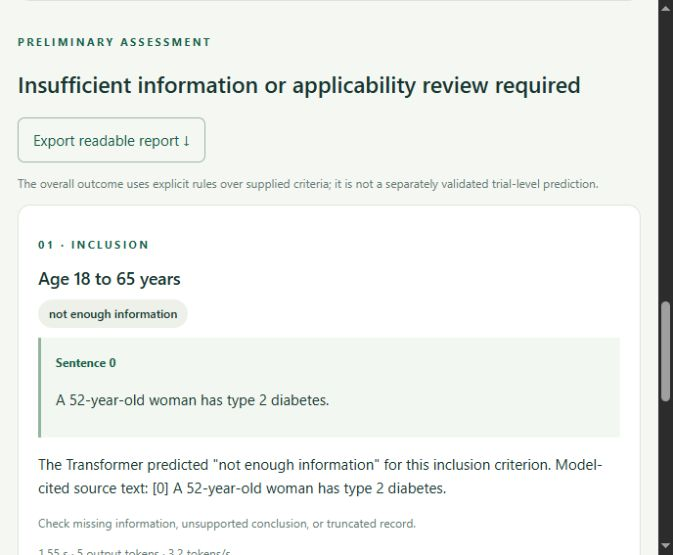
\includegraphics[width=\textwidth]{application.jpg}\caption{Genuine browser capture of the final CPU application on a synthetic record. The model abstains on an age criterion despite citing the stated age; this visible failure is preserved. The review warning and report-export control are part of the running interface.}\label{fig:app}\end{figure*}

Figure~\ref{fig:app} shows an actual model result, not a mockup. Empty-note and malformed-criterion errors were displayed, followed by successful recovery. Cached, uncached and speculative screening completed through browser controls with identical emitted tokens. The downloaded HTML report was opened in a browser and retained the synthetic record, citation, selected epoch and adapter fingerprint. The study-results tab displayed the saved held-out metrics. These functional checks do not validate clinical reasoning.

A browser-triggered live comparison used 151 input tokens and 16 raw output tokens, one warmup and two measured repeats per mode. Token equality passed. Mean total latency was 7.489 s uncached, 1.785 s cached, and 5.916 s speculative; draft acceptance was 0.0\%. This is a UI smoke comparison, separate from the controlled three-repeat benchmark tables.

Browser verification exposed a missing criterion-text value that serialized as NaN and prevented JavaScript from loading the trial selector. The application now filters invalid convenience-metadata entries; the benchmark split, annotations, frozen inference code and selected adapter were not changed. After correction, the browser populated the trial list and loaded selected criteria. A regression test rejects nonstandard JSON constants. The current full suite passes 22 checks, including the GPU-extension checks and this regression.

The live inference view exposes new measurements rather than a static performance chart; its additional screenshot accompanies the source as inference.jpg. Screenshot bytes were captured directly from the browser and saved unchanged; capture hashes and the verification record accompany the source.